\subsection{Segment-Onset Delay Signal}
The main timing feature uses a continuous piecewise-linear basis with knots at 2, 4, 6, and 10 seconds,
\begin{equation}
\begin{aligned}
\phi(d_s)={}&[d_s, (d_s-2)_+, (d_s-4)_+,\\
             &\phantom{[}(d_s-6)_+, (d_s-10)_+],
\end{aligned}
\end{equation}
where $(x)_+=\max(0,x)$. A dated protocol freeze records these knots before any model run reported in this study; available provenance does not establish that they preceded all inspection of the cohort. We therefore treat them as one fixed representation and compare linear, quadratic, log-delay, alternative-knot, quantile-knot, and binned sensitivities.

\subsection{Text-Derived Structural Features}
The deployable structural baseline uses source and interpreted-output lexical-unit counts, target/source length ratio, target punctuation and sentence-ending counts, target lexical diversity, a very-short-output indicator, and language direction. For Chinese, each CJK character is one lexical unit; for alphabetic text, each alphanumeric word is one unit. These features use no human score and are standardized inside each outer training fold. They test whether an apparent quality advantage is instead explained by output completeness, direction, or other readily observed properties of the interpreted output.

\subsection{Quality Signals}
The same-rubric human-quality reference uses $(q_s^{\mathrm{LQ}},q_s^{\mathrm{EXP}})$ and provides a related-rubric comparison unavailable to a deployed system. The automatic setting replaces it with $(\hat q_s^{\mathrm{LQ}},\hat q_s^{\mathrm{EXP}})$, where $\hat q_s=f_\theta(x_s)$ and $x_s$ is the ordered pair (source transcript, interpreted-output transcript). The frozen \texttt{Unbabel/wmt22-cometkiwi-da} backbone encodes the pair with the implementation tokenizer (512-token truncation, first-token pooling); two linear residual heads predict LQ and EXP. Official head-only runs use AdamW for ten fixed epochs (batch size 16) and fixed weighted MSE, variance, and correlation losses; checkpoint selection maximizes development LQ Pearson+EXP Pearson. The anonymous model card gives all weights, tokenizer fallback, architecture, and inference details.

Construction scripts trace generated alignment sets to source markdown and Whisper interpretation transcripts, but the normalized archive has no per-record record of transcription, punctuation, editing, or segmentation provenance across the full cohort. Tokenizer revision and token-length logs are also unavailable, so we do not reconstruct a truncation rate. The predictor consumes complete text pairs only and is post-hoc rather than streaming.

\subsection{Source-Speech-Group-Held-Out Evaluation}
For each held-out source-speech group $g$, all automatic predictions for $g$ come from an upstream quality model trained and selected only on other groups. Exact duplicate source-text--interpreted-output pairs from $g$ are removed from upstream train and development partitions. This protects the outer test group from quality-label leakage and tests transfer to unseen source content.

The second-stage promptness-training side is also cross-fitted. Within the remaining groups, four inner source-speech-group partitions generate out-of-fold $\hat q^{\mathrm{LQ}}$ and $\hat q^{\mathrm{EXP}}$ for every promptness-training row. A final outer-excluded quality model predicts group $g$. The second-stage Ridge regressor is trained on inner out-of-fold features and evaluated on the final outer prediction. Thus, no row's second-stage quality feature is produced by a model that used that row's LQ/EXP label.

The 16 outer folds and four inner partitions are deterministic greedy segment-count balances, with stable name tie-breaks and no direction/interpreter stratification. Each final fold holds one group out; inner held-out groups supply OOF predictions, and all seeds reuse the same manifest. Quality models run for fixed ten epochs without early stopping; checkpoint selection uses development LQ Pearson+EXP Pearson, while hyperparameters are fixed and outer-test labels are never used. Ridge scaling is fit on outer promptness-training rows only; PCA is diagnostic only. Outer test inputs are used solely to remove exact duplicate source--output pairs from upstream train/dev, never their labels. The manifest and row-count inventory are part of the planned camera-ready reproducibility release.

The full procedure is repeated for all 16 outer groups and the held-out predictions are concatenated before computing corpus-level metrics. The second-stage model is $\hat y_s=g_\beta([\hat q_s,\phi(d_s),\psi(x_s)])$, where $\psi$ denotes optional structural features. We compare $\phi(d)$ alone; structural features with delay; predicted LQ/EXP with delay; and their combination. Numeric features are standardized using only the promptness-training portion of each outer fold, and Ridge regularization is fixed at $\alpha=1.0$. Fixed-alpha sensitivity over OLS and $\alpha\in\{.01,.1,1,10,100\}$ is reported separately. The human row provides the same-rubric reference described above.

Because the target is bounded to $[.5,3.0]$ but Ridge is unbounded, we audit the primary predicted-quality-plus-delay system for each outer protocol and seed. We report counts below .5 and above 3.0, Pearson/Spearman, MSE, MAE, and calibration from the descriptive regression $y=a+b\hat y$. As sensitivity analyses, we post-hoc clip only the held-out prediction, $\mathrm{clip}(\hat y,.5,3.0)$, and fit a separate fold-local bounded continuous model $\hat y=.5+2.5\,\sigma(X\beta)$ with the same fixed $\ell_2$ penalty. The latter is fitted solely on each outer training fold; neither sensitivity uses outer-test labels. We also report the corresponding fold-training-mean predictor. These checks assess range and calibration robustness rather than select a new primary model.

\subsection{Interpreter-Disjoint Evaluation}
We additionally hold out each of the seven interpreters in turn. Every segment from the outer interpreter is excluded from quality training, development, checkpoint selection, and promptness-model training. Within the remaining interpreters, four inner speech-group partitions generate OOF predicted LQ/EXP for promptness-model training; a final interpreter-excluded quality model predicts the held-out interpreter. We compare delay-only, structural features with delay, predicted quality with delay, and their combination, with no interpreter identity or global-mean feature. Source speeches may still appear through other interpreters, so this protocol evaluates output from a held-out interpreter with possible source-content overlap; we report both pooled and interpreter-level behavior.

\subsection{Evaluator-Specific Construct Audit}
The rater analysis uses the same 16 source-speech-group outer folds but human labels rather than automatic quality predictions. For every ordered quality-rater--target-rater pair, the Ridge mapping is fitted directly on the outer-training groups using the stated rater's LQ/EXP and shared segment-onset-delay features as inputs and the stated target rater's professional promptness ratings as outcomes. The fitted mapping is then evaluated on the held-out group's inputs from that same quality rater and outcomes from that same target rater. Thus, R05-quality$\rightarrow$R06-promptness and R06-quality$\rightarrow$R05-promptness are distinct target-specific models; no held-out target labels enter fitting or scaling.

\begin{figure*}[t]
\centering
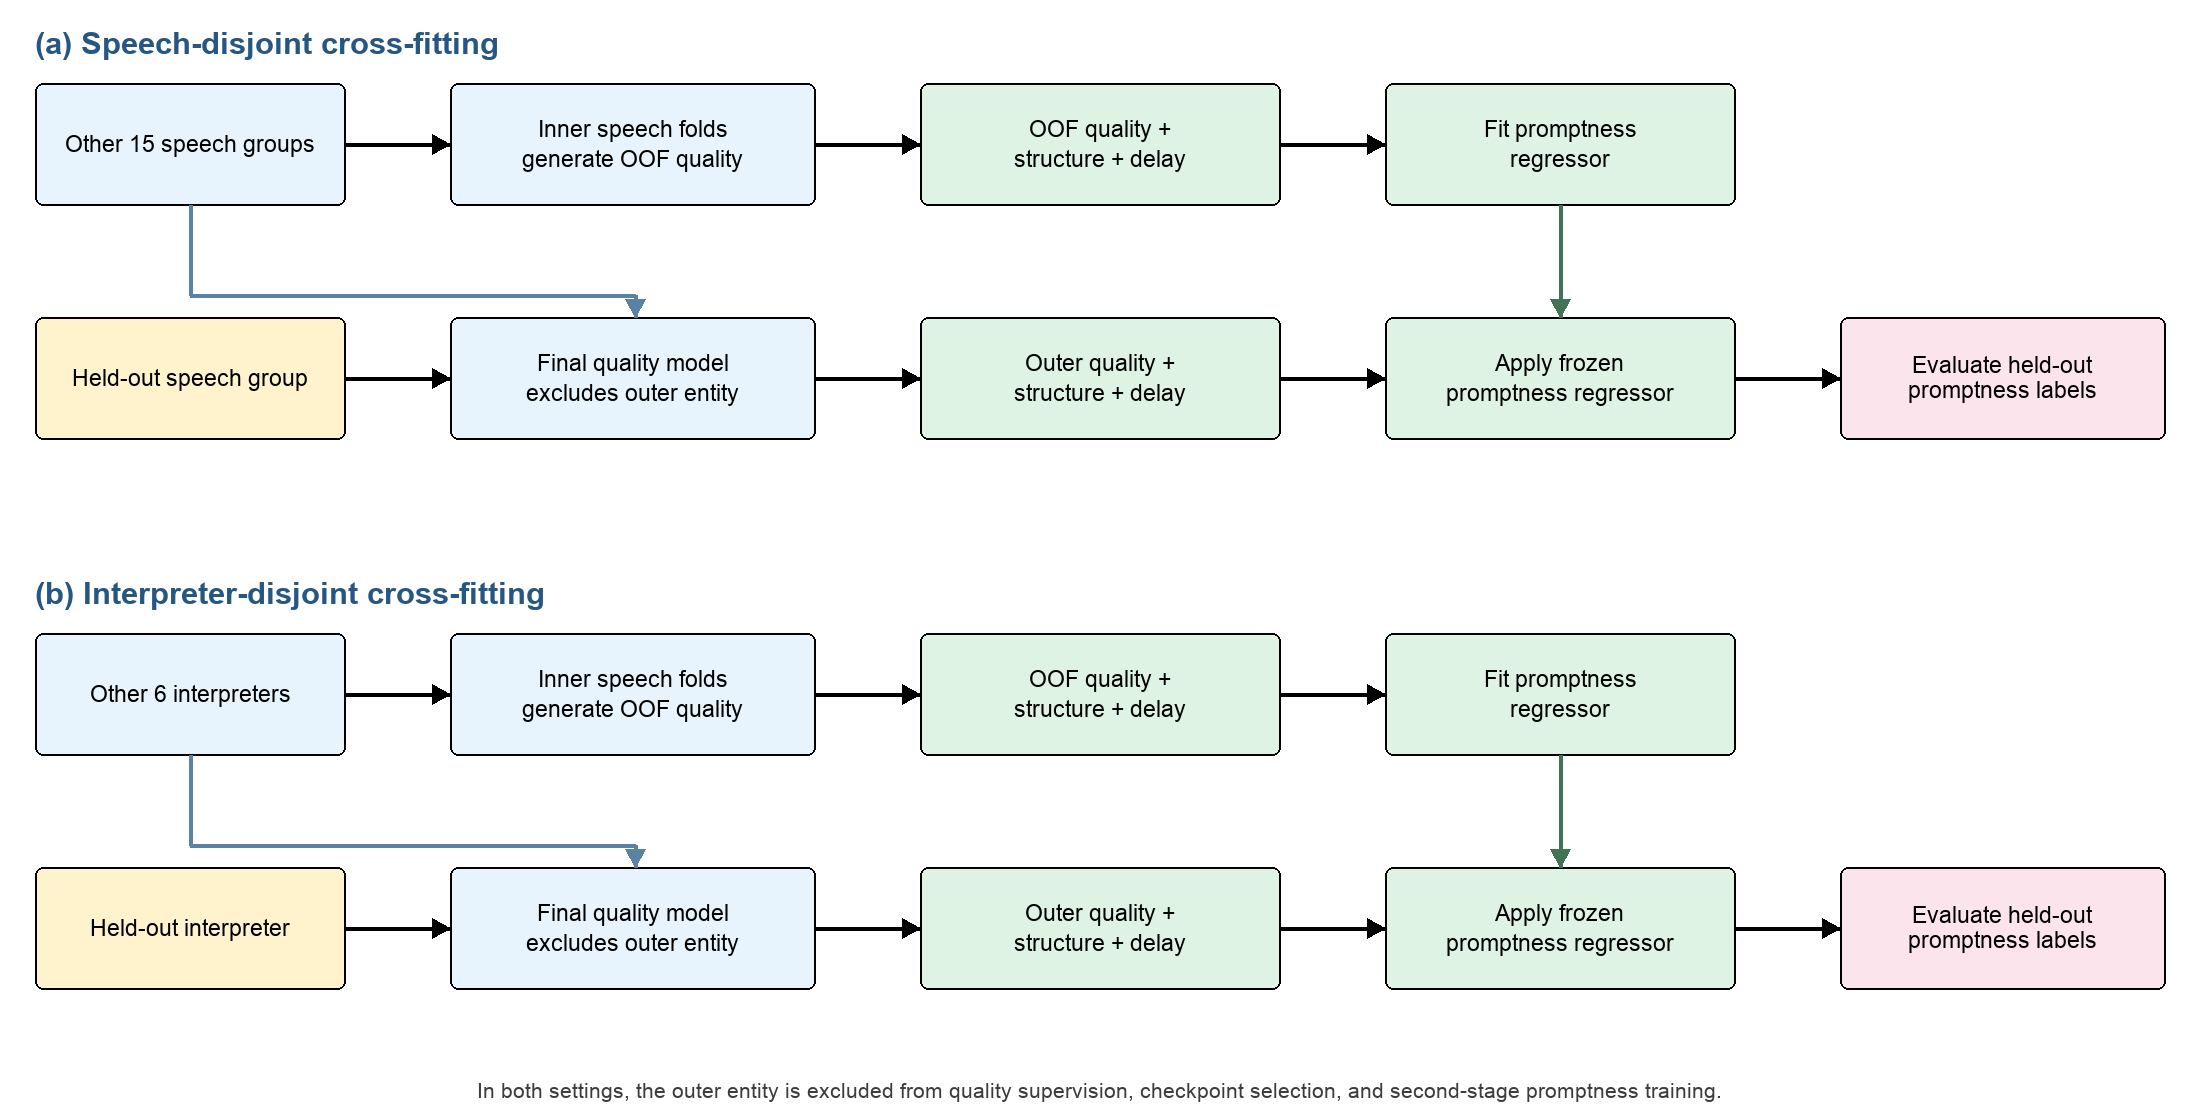
\includegraphics[width=.96\textwidth]{figures/fig_method_pipeline.png}
\caption{Cross-fitted two-stage protocols. Panel (a) holds out a speech group; panel (b) holds out an interpreter. In both settings the outer entity is excluded from quality supervision, checkpoint selection, and second-stage promptness-model training.}
\label{fig:pipeline}
\end{figure*}

\subsection{Uncertainty and Decision Rule}
Automatic point estimates are means over three fixed training seeds; their reported $\pm$ values are sample SDs across those seeds, not sampling confidence intervals. For source-speech-group-held-out results, we use 10,000 cluster-bootstrap draws: we resample the 16 source-speech groups with replacement, and each selected group contributes all of its segments. In every draw, we calculate each metric separately for each seed and then average it, matching the main-table point-estimate convention. The table delta averages seed-level correlations; the permutation uses segment-wise seed-mean predictions, so its system-level statistic differs because Pearson is nonlinear. We apply the identical group draw to paired systems to obtain CIs for their metric differences.

We define two comparisons. The \emph{primary prespecified comparison}, predicted quality+delay versus timing-only, tests the task's construct-level hypothesis that cross-fitted professional-quality signals add information beyond segment-onset delay. Its statistic is $T=r(y,\hat y_{Q+D})-r(y,\hat y_D)$. We enumerate all $2^{16}=65{,}536$ whole-group label swaps, preserve unequal observed group sizes in corpus correlation, use a two-sided alternative, and apply plus-one correction $p=(1+\#\{|T^*|\geq|T|\})/(1+65{,}536)$. The stricter secondary comparison, full versus structural+delay, asks whether predicted quality adds information beyond deterministic structure and timing. We report its paired cluster-bootstrap intervals and per-seed/group distributions descriptively, without another $p$-value. Seed-wise swaps and interpreter-disjoint results are descriptive. We report prediction SDs to detect collapse.
